\chapter{Model selection}\label{chapter:model_selection}

Chapter \ref{chapter:robustness_assessment} explored the robustness assessment
capabilities of the PA kernel in image classification tasks and provided extensive 
evidence of its suitability as an algorithm selection criterion in covariate shift settings. 
This chapter extends our previous findings by investigating 
how the PA kernel can be leveraged for robust epoch-wise model selection
with early stopping, potentially enhancing
generalization performance under distribution shifts. \\

It is important to recognize that epoch-wise model selection represents a fundamentally 
different paradigm from the robustness assessment framework discussed in 
the previous chapter, which could be described as algorithm selection. In 
the previous scenario, models were selected based on standard validation accuracy and subsequently 
evaluated for their robustness to different sources of covariate shift. 
The assessment was thus conducted on a configuration of weights that had already been selected to
encode a suitable inductive bias that demonstrated to perform well on samples drawn
from the same distribution. \\

In that context, the robustness assessment provided by PA was implicitly constrained to a 
definition of generalization error that could be assumed to align with the error associated to
the task performance, and predictions were expected to match the desired learning outcome.
However, this assumption breaks down when extending the evaluation framework to 
epoch-wise selection, as consistency in predictive outcomes across different samples does not 
guarantee alignment with the performance over the task at hand. More specifically,
there is no assurance that the inductive bias encoded by the most robust model actually
represents a set of features that are relevant to the learning problem. \\

This reasoning becomes clearer when the problem is formulated in a data-agnostic way. % from a data-agnostic perspective. 
After every epoch, the classifier encodes a different feature extractor function $\Phi$, resulting 
in distinct feature space vectors for each observation. Every epoch can therefore be considered as
an independent sampling experiment in the feature space, and robustness between 
two realizations of these experiments is then evaluated using PA. Given that the 
underlying statistical model governing the sampling process is determined by the inductive 
bias of the model, which varies at every epoch, it is not possible for PA to mitigate or even detect
overfitting to suboptimal biases associated with features or spurious correlations that are also
present in the samples it relies upon. \\

Overall, the critical distinction between performance-based and robustness-based criteria 
has already been addressed, more notably in Section \ref{sec:results_robustness}.
It is clear that a classifier overfitting to specific features in the training data
would lower its performance in validation data and simultaneously be considered
increasingly robust. Besides, the ultimate measure of success in model selection will remain
to be accuracy on test sets, particularly those from the target domain, as this is the primary
objective of domain adaptation.  \\

For these reasons, this chapter will explore two principal situations. First, the potential 
misalignment between robustness measurement and task performance will be monitored by 
considering a wide range of validation sample pairs for a single learning task. In most cases, 
$\bm{x}^\prime$ will be drawn from a source environment and thus encode a set of features that 
the model has seen during training, while $\bm{x}^{\prime \prime}$ will be drawn from target 
environments. In particular, different levels of shift will be considered for $\bm{x}^{\prime \prime}$,
as to simulate different degrees of access to target domains. The loss minimization process will 
ensure that the model's predictions for $\bm{x}^\prime$ align with the desired learning outcomes
and, in turn, robustness assessment will evaluate whether predictions for $\bm{x}^{\prime \prime}$ 
align with these expectations as well. The ability of the robustness criterion to select models
that perform well in target domains will be in question. \\

Second, the behavior and suitability of robustness metrics as model selection criteria
will be assessed under specific configurations of the training data that are crafted to
encode suboptimal sets of features in the inductive bias. In particular, several degrees of
co-occurence between image factors and output labels will be introduced, and the model 
selection capabilities of PA will be compared to that of standard 
accuracy under these conditions.

\section{DiagVib-6 Benchmark}\label{chapter:msel_controlled}

Building upon the exploratory results in the out-of-distribution setting, 
the robust model selection capabilities of PA will be assessed across a
wide range of distribution shift conditions in a controlled experimental setup. In particular,
different shift factors will be considered for both source environments and target 
environments. These findings will help identify the experimental conditions in which the 
discriminative power of PA is most effective. \\

Experiments have been conducted in a similar setting to that of \textbf{Experiment 5a-5b}, 
with a reduced dataset size to avoid repetition of MNIST 
observations. This ensures that each training observation uniquely represents a specific instance 
of the number drawing experiment, along with the corresponding domain 
shift perturbation. Given that factor modifications are not deterministic, this approach prevents the model's inductive bias 
from being influenced by an implicit data augmentation process.

\paragraph{Experiment 6.} Model selection experiments in the domain generalization setting 
have been conducted within the DiagVib-6 \cite{euligDiagViB6DiagnosticBenchmark2021}
data generation pipeline, which
was already described in Section \ref{results_domain_generalization}. ERM, 
IRM \cite{arjovskyInvariantRiskMinimization2020}
and
LISA \cite{yaoImprovingOutofDistributionRobustness2022}
algorithms have been used to train a ResNet18 for 100 epochs on source environments through
SGD \cite{ruderOverviewGradientDescent2017} 
and Adam \cite{kingmaAdamMethodStochastic2017}
optimizers with learning rates $5 \times 10^{-5}$,  $10^{-4}$, $5 \times 10^{-4}$ and $10^{-3}$. 
For each case, model validation and selection has been conducted on increasingly
shifted datasets, encompassing both target and source domains, by storing the weights
that displayed the best performance on different metrics. More specifically, 
PA, AFR$_{\text{P}}$ and accuracy on validation datasets have been computed every epoch
and used as early stopping criteria. \\

The characterization of the inductive bias is outside of the scope of this work, but given the
triviality of the experimental setup and the learning task associated, it is reasonable to assume 
that it encompasses all the relevant features that are present in the data,
including the randomness instantiation, the nature of the shift and their relative frequency in the
data. The optimization process will iteratively navigate the loss landscape and implicitly
balance these features differently, leading to different predictive outcomes.  \\

In this regard, two primary sources of inductive bias were examined by varying the nature of the
shift defining the two source environments, namely based on the hue factor, as was the case in the
previous chapter, and based on the position factor. These represent the two most significant 
sources of variability from an image representation perspective, and comparing the model selection 
capabilities across these settings will provide insight into the consistency of the criteria. \\

For this experiment, two sampling instantiations $\tau_0^{\text{val}} \neq \tau_1^{\text{val}}$ 
are considered for the validation datasets, which means that $\bm{x}_0^{\text{val}}$ and $\bm{x}_1^{\text{val}}$ 
entail different instantiations of the shift factor and the sampling experiment. 
Table \ref{ds:hue_trainval} and Table \ref{ds:pos_trainval} specify 
the configuration of factors considered for the training and validation datasets. In the former,
source domains are shifted in the hue factor, while in the latter the position factor is considered.

\begin{dataset}[Training and validation \texttt{hue}]
    Training datasets are always drawn from source domains. More specifically, they are composed of samples 
    $\bm{x}_0^{\text{train}} \circ \tau_0^{\text{train}}$ and $\bm{x}_1^{\text{train}} \circ \tau_1^{\text{train}}$, 
    with $\tau_0^{\text{train}} \neq \tau_1^{\text{train}}$. Validation datasets are composed of samples
    $\bm{x}_0^{\text{val}} \circ \tau_0^{\text{val}}$, $\bm{x}_1^{\text{val}} \circ \tau_1^{\text{val}}$,
    $\tau_0^{\text{val}} \neq \tau_1^{\text{val}}$, which are either drawn from source domains, target domains or a combination of both.

    \begin{itemize}
        \item When both $\bm{x}_0^{\text{val}}, \bm{x}_1^{\text{val}}$ are drawn from source domains, 
        two configurations are considered, namely when they are drawn from the same distribution (SD) and when 
        they are not, in which case are still defined in-distribution (ID) with respect to training samples.
        \item When $\bm{x}_0^{\text{val}}$ is drawn from the source and $\bm{x}_1^{\text{val}}$ is drawn
        from target domains, two more configurations are considered. In particular, depending on the magnitude of the 
        shift entailed by $\bm{x}_1^{\text{val}}$, 1-factor mixed distribution (1F-MD) and 5-factor mixed 
        distribution (5F-MD) samples can be considered. The former entails a shift in the factor that defines the
        experiment (i.e. hue), while the latter considers a scenario in which all possible factors are shifted.
        \item When both $\bm{x}_0^{\text{val}}, \bm{x}_1^{\text{val}}$ are drawn from target domains, 
        a single out-of-distribution (OOD) configuration is considered, where both samples entail a different
        instantiation in the factor that defines the experiment.
    \end{itemize}

    \begin{table}[H]
        \centering
        \begin{tabular}{c|c|c|c|c|c|c|c}
             & Env. & Hue & Lightness & Position & Scale & Texture & \textit{Shape} \\
            \specialrule{1.5pt}{1pt}{1pt}  % Thicker line
            \multirow{2}{*}{Training} 
            & 0 & red & dark & CC & large & blank & \textit{1,4,7,9} \\
            & 1 & \textbf{blue} & dark & CC & large & blank & \textit{1,4,7,9} \\
            \specialrule{1.5pt}{1pt}{1pt}  % Thicker line
            \multirow{1}{*}{Validation} 
            & 0 & red & dark & CC & large & blank & \textit{1,4,7,9} \\
            \hline
            \multirow{1}{*}{SD} 
            & 1 & red & dark & CC & large & blank & \textit{1,4,7,9} \\
            \multirow{1}{*}{ID} 
            & 1 & \textbf{blue} & dark & CC & large & blank & \textit{1,4,7,9} \\
            \multirow{1}{*}{1F-MD} 
            & 1 & \textbf{magenta} & dark & CC & large & blank & \textit{1,4,7,9} \\
            \multirow{1}{*}{5F-MD} 
            & 1 & \textbf{green} & \textbf{bright} & \textbf{UL} & \textbf{small} & \textbf{tiles} & \textit{1,4,7,9} \\
            \specialrule{1.5pt}{1pt}{1pt}  % Thicker line
            \multirow{2}{*}{Validation OOD} 
            & 0 & \textbf{yellow} & dark & CC & large & blank & \textit{1,4,7,9} \\
            & 1 & \textbf{magenta} & dark & CC & large & blank & \textit{1,4,7,9} \\
            \specialrule{1.5pt}{1pt}{1pt}  % Thicker line
        \end{tabular}
        \caption{
        Image factors associated with each of the environments considered in this experiment. CC and UL account
        for 'centered center' and 'upper left', respectively.
        }
        \label{ds:hue_trainval}
    \end{table}
\end{dataset}

\begin{dataset}[Test \texttt{hue}] Source domains are shifted in the hue factor. Consequently,
    target domains entailed incremental shifts in the remaining factors.

    \begin{table}[H]
        \centering
        \begin{tabular}{l|c|c|c|c|c|c}
        \# Factors & 0 & 1 & 2 & 3 & 4 & 5 \\
        \midrule
        Hue & red & \textbf{green} & green & green & green & green \\
        Lightness & dark & dark & \textbf{bright} & bright & bright & bright \\
        Position  & CC & CC & CC & CC & \textbf{UL} & UL \\
        Scale  & large & large & large & large & large & \textbf{small} \\
        Texture & blank & blank & blank & \textbf{tiles} & tiles & tiles \\
        \textit{Shape} & \textit{1,4,7,9} &  \textit{1,4,7,9} &  \textit{1,4,7,9} & \textit{1,4,7,9} & \textit{1,4,7,9} & \textit{1,4,7,9} \\
        \bottomrule
        \end{tabular}
        \caption{
        Image factors associated to each of the environments considered in this experiment. CC and UL account
        for 'centered center' and 'upper left', respectively.
        }
        \label{ds:hue_test}
    \end{table}
\end{dataset}

For each validation dataset configuration, task performance (i.e. accuracy) will be reported on 
progressively shifted test datasets, as outlined in Table \ref{ds:hue_test}
for the hue factor and Table \ref{ds:pos_test} for the position factor experiments. Specifically, 
results will be associated with the optimization process that achieved the highest aggregated test accuracy 
across all the datasets. In other words, the optimization configuration that maximizes 
the cumulative performance across all test datasets will be reported, regardless of the 
model selection criterion. Under these conditions, only the best-performing models 
will be considered, allowing for a focused assessment of the suitability of the 
model selection criteria. \\

Tables \ref{tab:dg_hue_notpaired}-\ref{tab:dg_pos_notpaired} display the test performance of the selected 
models across different dataset configurations and model selection criteria. A key observation is that 
models trained under a shift in the hue factor (Table \ref{tab:dg_hue_notpaired}) exhibit significantly 
lower performance compared to those trained under a shift in the position factor (Table \ref{tab:dg_pos_notpaired}).
This performance discrepancy is particularly noticeable in the first shifted test dataset, which contains the same configuration
of factors in both experiments and shows a clear performance gap between the two. \\

Test datasets encode cumulative shifts, and each of them potentially favors specific features 
in the model's inductive bias. Consequently, models that demonstrate significant performance improvements 
in some datasets when selected using PA may exhibit the opposite behavior in others. Due to this variability, aggregated performance has been adopted as an experimental 
criterion to provide a more comprehensive evaluation, and the suitability of a selection metric will be
determined based on its consistency across different datasets, not on a particular one. \\

Both experiments reveal a strong alignment in the model selection capabilities of validation accuracy and 
$\operatorname{AFR}_{\text{P}}$. As described in previous chapters, accuracy provides an assessment based on 
task performance, while $\operatorname{AFR}_{\text{P}}$ serves as our baseline robustness metric, thus accounting for 
changes in performance under distribution shifts. The strong alignment in their model selection capabilities is a significant 
observation, as it underscores that the discriminative power driving PA is fundamentally different from that of 
accuracy-based metrics. \\

\begin{table}[H]
    \centering
    \setlength{\tabcolsep}{2.5pt}
    \resizebox{\textwidth}{!}{%
    \begin{tabular}{l|ccc|ccc|ccc|ccc|ccc|ccc}
    \multirow{3}{*}{} & \multicolumn{3}{c|}{\textbf{Acc. Test 0}} & \multicolumn{3}{c|}{\textbf{Acc. Test 1}} & \multicolumn{3}{c|}{\textbf{Acc. Test 2}} & \multicolumn{3}{c|}{\textbf{Acc. Test 3}} & \multicolumn{3}{c|}{\textbf{Acc. Test 4}} & \multicolumn{3}{c}{\textbf{Acc. Test 5}} \\
    \textbf{{\color{tab:blue} \textbf{ERM}}} & Acc. & AFR$_\text{P}$ & PA & Acc. & AFR$_\text{P}$ & PA & Acc. & AFR$_\text{P}$ & PA & Acc. & AFR$_\text{P}$ & PA & Acc. & AFR$_\text{P}$ & PA & Acc. & AFR$_\text{P}$ & PA \\
    \midrule
    SD & 99.4 & 99.4 & {\textbf{99.5}} & 42.1 & 42.1 & {\textbf{55.0}} & {\textbf{70.4}} & \textbf{70.4} & 69.7 & 68.0 & 68.0 & {\textbf{68.3}} & 52.6 & 52.6 & {\textbf{52.7}} & {\textbf{41.7}} & \textbf{41.7} & 30.2 \\
    ID & {\textbf{99.5}} & \textbf{99.5} & 99.4 & 49.6 & 49.6 & {\textbf{69.3}} & {\textbf{90.2}} & \textbf{90.2} & 87.3 & 81.0 & 81.0 & {\textbf{82.1}} & {\textbf{71.4}} & \textbf{71.4} & 69.6 & {\textbf{44.6}} & \textbf{44.6} & 39.0 \\
    1F-MD & 99.3 & 99.3 & 99.3 & 47.4 & 47.4 & 47.4 & 78.6 & 78.6 & 78.6 & 70.7 & 70.7 & 70.7 & 63.7 & 63.7 & 63.7 & 36.7 & 36.7 & 36.7 \\
    5F-MD & 99.5 & 99.5 & 99.5 & 49.6 & 49.6 & 49.6 & 90.2 & 90.2 & 90.2 & 81.0 & 81.0 & 81.0 & 71.4 & 71.4 & 71.4 & 44.6 & 44.6 & 44.6 \\
    OOD & 99.3 & 99.3 & 99.3 & 60.9 & 60.9 & 60.9 & 92.6 & 92.6 & 92.6 & 83.9 & 83.9 & 83.9 & 64.9 & 64.9 & 64.9 & 32.3 & 32.3 & 32.3 \\
    \midrule
    \addlinespace
    \addlinespace
    \textbf{{\color{tab:orange} \textbf{IRM}}} & Acc. & AFR$_\text{P}$ & PA & Acc. & AFR$_\text{P}$ & PA & Acc. & AFR$_\text{P}$ & PA & Acc. & AFR$_\text{P}$ & PA & Acc. & AFR$_\text{P}$ & PA & Acc. & AFR$_\text{P}$ & PA \\
    \midrule
    SD & 99.3 & 99.3 & 99.3 & 71.5 & 71.5 & {\textbf{83.3}} & 70.6 & 70.6 & {\textbf{91.9}} & 65.3 & 65.3 & {\textbf{85.9}} & {\textbf{75.0}} & \textbf{75.0} & 66.5 & 28.8 & 28.8 & {\textbf{46.7}} \\
    ID & 99.4 & 99.4 & 99.4 & 44.3 & 44.3 & 44.3 & 88.1 & 88.1 & 88.1 & 76.1 & 76.1 & 76.1 & 59.4 & 59.4 & 59.4 & 45.2 & 45.2 & 45.2 \\
    1F-MD & 99.4 & 99.4 & 99.4 & 44.3 & 44.3 & 44.3 & 88.1 & 88.1 & 88.1 & 76.1 & 76.1 & 76.1 & 59.4 & 59.4 & 59.4 & 45.2 & 45.2 & 45.2 \\
    5F-MD & {\textbf{99.4}} & \textbf{99.4} & 99.3 & 31.2 & 31.2 & {\textbf{83.3}} & 88.7 & 88.7 & {\textbf{91.9}} & 73.8 & 73.8 & {\textbf{85.9}} & 65.5 & 65.5 & {\textbf{66.5}} & {\textbf{50.2}} & \textbf{50.2} & 46.7 \\
    OOD & 99.5 & 99.5 & 99.5 & 62.4 & 62.4 & 62.4 & 90.1 & 90.1 & 90.1 & 84.1 & 84.1 & 84.1 & 52.2 & 52.2 & 52.2 & 42.6 & 42.6 & 42.6 \\
    \midrule
    \addlinespace
    \addlinespace
    \textbf{{\color{tab:green} \textbf{LISA}}} & Acc. & AFR$_\text{P}$ & PA & Acc. & AFR$_\text{P}$ & PA & Acc. & AFR$_\text{P}$ & PA & Acc. & AFR$_\text{P}$ & PA & Acc. & AFR$_\text{P}$ & PA & Acc. & AFR$_\text{P}$ & PA \\
    \midrule
    SD & 99.3 & 99.3 & {\textbf{99.4}} & {\textbf{88.4}} & \textbf{88.4} & 83.1 & 53.9 & 53.9 & {\textbf{78.5}} & 57.9 & 57.9 & {\textbf{80.5}} & 63.1 & 63.1 & {\textbf{77.0}} & {\textbf{38.8}} & \textbf{38.8} & 35.4 \\
    ID & 99.5 & 99.5 & 99.5 & 59.2 & 59.2 & {\textbf{88.8}} & {\textbf{62.5}} & \textbf{62.5} & 60.4 & 71.7 & 71.7 & {\textbf{76.8}} & 70.9 & 70.9 & {\textbf{71.5}} & 35.2 & 35.2 & {\textbf{36.4}} \\
    1F-MD & 99.5 & 99.5 & 99.5 & 88.8 & 88.8 & 88.8 & 54.4 & 54.4 & 54.4 & 76.8 & 76.8 & 76.8 & 71.5 & 71.5 & 71.5 & 36.4 & 36.4 & 36.4 \\
    5F-MD & 99.2 & 99.2 & {\textbf{99.4}} & {\textbf{86.6}} & \textbf{86.6} & 85.1 & 71.1 & 71.1 & {\textbf{74.8}} & 77.3 & 77.3 & {\textbf{83.7}} & 73.7 & 73.7 & {\textbf{81.9}} & {\textbf{49.4}} & \textbf{49.4} & 48.6 \\
    OOD & {\textbf{99.3}} & 99.2 & 99.2 & 91.8 & {\textbf{95.8}} & 84.4 & 59.0 & 63.0 & {\textbf{83.0}} & 77.6 & 79.0 & {\textbf{88.0}} & 73.8 & 73.6 & {\textbf{84.8}} & 34.4 & 40.4 & {\textbf{47.3}} \\
    \bottomrule
\end{tabular}%
}
\caption{
    Test performance under increasing levels of shift for models selected through different configurations of 
    validation datasets. PA, AFR$_{\text{P}}$ and accuracy are used as early stopping criteria for model selection
    in the hue factor experiment (see Tables \ref{ds:hue_trainval}-\ref{ds:hue_test}).}
\label{tab:dg_hue_notpaired}
\end{table}

\begin{table}[H]
\centering
\setlength{\tabcolsep}{2.5pt}
\resizebox{\textwidth}{!}{%
\begin{tabular}{l|ccc|ccc|ccc|ccc|ccc|ccc}
\multirow{3}{*}{} & \multicolumn{3}{c|}{\textbf{Acc. Test 0}} & \multicolumn{3}{c|}{\textbf{Acc. Test 1}} & \multicolumn{3}{c|}{\textbf{Acc. Test 2}} & \multicolumn{3}{c|}{\textbf{Acc. Test 3}} & \multicolumn{3}{c|}{\textbf{Acc. Test 4}} & \multicolumn{3}{c}{\textbf{Acc. Test 5}} \\
\textbf{{\color{tab:blue} \textbf{ERM}}} & Acc. & AFR$_\text{P}$ & PA & Acc. & AFR$_\text{P}$ & PA & Acc. & AFR$_\text{P}$ & PA & Acc. & AFR$_\text{P}$ & PA & Acc. & AFR$_\text{P}$ & PA & Acc. & AFR$_\text{P}$ & PA \\
\midrule
SD & 99.5 & 99.5 & 99.5 & {\textbf{99.5}} & \textbf{99.5} & 99.4 & {\textbf{85.7}} & \textbf{85.7} & 84.7 & 42.0 & 42.0 & {\textbf{66.3}} & 45.0 & 45.0 & {\textbf{51.4}} & 38.5 & 38.5 & {\textbf{51.8}} \\
ID & 99.3 & 99.3 & {\textbf{99.4}} & {\textbf{99.5}} & \textbf{99.5} & 99.4 & 84.9 & 84.9 & {\textbf{86.6}} & 66.3 & 66.3 & {\textbf{68.9}} & {\textbf{52.0}} & \textbf{52.0} & 50.2 & 46.3 & 46.3 & {\textbf{48.1}} \\
1F-MD & 99.3 & 99.3 & {\textbf{99.4}} & {\textbf{99.5}} & \textbf{99.5} & 99.4 & 84.9 & 84.9 & {\textbf{86.6}} & 66.3 & 66.3 & {\textbf{68.9}} & {\textbf{52.0}} & \textbf{52.0} & 50.2 & 46.3 & 46.3 & {\textbf{48.1}} \\
5F-MD & {\textbf{99.6}} & \textbf{99.6} & 99.1 & {\textbf{99.4}} & \textbf{99.4} & 99.1 & 84.3 & 84.3 & {\textbf{90.1}} & {\textbf{65.2}} & 65.2 & 58.6 & 66.2 & 66.2 & {\textbf{73.3}} & 57.4 & 57.4 & \textbf{57.6} \\
OOD & {\textbf{99.5}} & \textbf{99.5} & 99.4 & {\textbf{99.5}} & \textbf{99.5} & 99.4 & {\textbf{87.0}} & \textbf{87.0} & 86.6 & {\textbf{75.1}} & \textbf{75.1} & 68.9 & {\textbf{56.9}} & \textbf{56.9} & 50.2 & {\textbf{57.5}} & \textbf{57.5} & 48.1 \\
\midrule
\addlinespace
\addlinespace
\textbf{{\color{tab:orange} \textbf{IRM}}} & Acc. & AFR$_\text{P}$ & PA & Acc. & AFR$_\text{P}$ & PA & Acc. & AFR$_\text{P}$ & PA & Acc. & AFR$_\text{P}$ & PA & Acc. & AFR$_\text{P}$ & PA & Acc. & AFR$_\text{P}$ & PA \\
\midrule
SD & 99.2 & 99.2 & {\textbf{99.5}} & 99.4 & 99.4 & {\textbf{99.5}} & 83.3 & 83.3 & {\textbf{89.9}} & 43.5 & 43.5 & \textbf{44.3} & 53.4 & 53.4 & {\textbf{59.0}} & 44.6 & 44.6 & {\textbf{48.2}} \\
ID & 99.3 & 99.3 & 99.3 & 99.5 & 99.5 & 99.5 & 77.7 & 77.7 & 77.7 & 57.4 & 57.4 & 57.4 & 55.9 & 55.9 & 55.9 & 50.4 & 50.4 & 50.4 \\
1F-MD & 99.3 & 99.3 & 99.3 & 99.5 & 99.5 & 99.5 & {\textbf{84.6}} & \textbf{84.6} & 77.7 & {\textbf{69.8}} & \textbf{69.8} & 57.4 & {\textbf{64.4}} & \textbf{64.4} & 55.9 & {\textbf{57.5}} & \textbf{57.5} & 50.4 \\
5F-MD & 98.8 & 98.8 & 98.8 & 98.8 & 98.8 & 98.8 & 84.6 & 84.6 & 84.6 & 81.8 & 81.8 & 81.8 & 69.5 & 69.5 & 69.5 & 63.1 & 63.1 & 63.1 \\
OOD & 99.3 & 99.3 & 99.3 & 99.5 & 99.5 & 99.5 & 84.6 & 84.6 & 84.6 & 69.8 & 69.8 & 69.8 & 64.4 & 64.4 & 64.4 & 57.5 & 57.5 & 57.5 \\
\midrule
\addlinespace
\addlinespace
\textbf{{\color{tab:green} \textbf{LISA}}} & Acc. & AFR$_\text{P}$ & PA & Acc. & AFR$_\text{P}$ & PA & Acc. & AFR$_\text{P}$ & PA & Acc. & AFR$_\text{P}$ & PA & Acc. & AFR$_\text{P}$ & PA & Acc. & AFR$_\text{P}$ & PA \\
\midrule
SD & 99.3 & 99.3 & 99.3 & 99.4 & 99.4 & 99.4 & 85.3 & 85.3 & 85.3 & 56.5 & 56.5 & 56.5 & 53.9 & 53.9 & 53.9 & 44.2 & 44.2 & 44.2 \\
ID & {\textbf{99.5}} & \textbf{99.5} & 99.3 & 99.3 & 99.3 & {\textbf{99.4}} & 62.3 & 62.3 & {\textbf{85.3}} & 50.6 & 50.6 & {\textbf{56.5}} & 52.9 & 52.9 & {\textbf{53.9}} & 42.9 & 42.9 & {\textbf{44.2}} \\
1F-MD & 99.3 & 99.3 & 99.3 & 99.4 & 99.4 & 99.4 & 85.3 & 85.3 & 85.3 & 56.5 & 56.5 & 56.5 & 53.9 & 53.9 & 53.9 & 44.2 & 44.2 & 44.2 \\
5F-MD & {\textbf{99.3}} & \textbf{99.3} & 99.0 & {\textbf{99.2}} & \textbf{99.2} & 99.1 & {\textbf{80.0}} & \textbf{80.0} & 77.5 & {\textbf{88.6}} & \textbf{88.6} & 77.2 & 68.4 & 68.4 & {\textbf{73.7}} & 64.5 & 64.5 & 64.5 \\
OOD & {\textbf{99.5}} & \textbf{99.5} & 99.3 & 99.3 & 99.3 & {\textbf{99.4}} & 62.3 & 62.3 & {\textbf{85.3}} & 50.6 & 50.6 & {\textbf{56.5}} & 52.9 & 52.9 & {\textbf{53.9}} & 42.9 & 42.9 & {\textbf{44.2}} \\
\bottomrule
\end{tabular}%
}
\caption{Test performance under increasing levels of shift for models selected through different configurations of 
validation datasets. PA, AFR$_{\text{P}}$ and accuracy are used as early stopping criteria for model selection
in the position factor experiment (see Tables \ref{ds:pos_trainval}-\ref{ds:pos_test}).
}
\label{tab:dg_pos_notpaired}
\end{table}

Overall, models selected through PA demonstrate equal or superior performance under increasing levels of domain shift. 
In particular, ID and SD dataset configurations, which address the domain adaptation problem for being limited
to source-related factor configurations, show substantial improvements compared to those chosen by 
accuracy-based metrics. When PA-based selection underperforms, it does so by a small margin, whereas in cases where it outperforms, the 
margin of improvement is much larger. \\

Alternative results were obtained using the same factor configuration but with a single instantiation of 
the sampling experiment $\tau^{\text{val}}$, in a way that samples $\bm{x}_0^{\text{val}}$ and $\bm{x}_1^{\text{val}}$
are composed of the same MNIST observations. Tables \ref{tab:dg_hue_paired}-\ref{tab:dg_pos_paired} present these
results, from which no conclusive evidence can be drawn. More specifically, accuracy and $\operatorname{AFR}_{\text{P}}$ are
not aligned in their selection of models, and neither of the metrics provides a consistent 
superior model selection capabilities. \\

These experiments yield some important and a priori counterintuitive conclusions. First, they demonstrate 
that PA is more effective for model selection in the presence of sampling randomness; that is, when posterior 
agreement is maximized between different observations of the same class. One might intuitively expect that 
filtering out sampling randomness would lead to selecting a model encoding the most robust set of features
with respect to the distribution shift, and that these features would be proven to generalize under
target domain shifts, regardless of the particular sampling instance. However, these results suggest that 
different instances of the same class improve PA model selection performance, even when source 
environments are accounted for in validation and overfitting to irrelevant features is mitigated. Besides, 
PA is shown to be more effective in in-distribution model selection settings (i.e. ID and SD), and does not always 
outperform accuracy-based metrics in mixed-distribution or out-of-distribution scenarios, at least in the
ERM and IRM cases. \\

\newpage

\section{In-distribution DiagVib-6}

Thus far, experiments in the domain generalization setting have been conducted 
under synthetic conditions, where the effect of the shift was uniform across the sample and the 
presence of predictive and non-predictive factors was balanced.  These experiments have 
demonstrated that PA successfully discriminates robust from non-robust learners and also provides 
increased early-stopping performance compared with current baseline metrics, particularly in
domain adaptation conditions. \\

However, real-world datasets are subject to heteroscedastic sources of sampling randomness 
and often exhibit feature distributions that are severely misaligned with the true distribution 
in the sample space, which is commonly known as subpopulation shifts. This section aims to reproduce these conditions 
by considering controlled environments where the presence of certain image factors is deliberately 
manipulated to induce an inductive bias towards suboptimal feature representations. These representations 
may generalize well to sampling variability within source environments but fail to adapt to 
distribution shifts in target environments, which poses an additional challenge to
the domain adaptation problem. 

\paragraph{Experiment 7.}\label{def:zso_theory}
    Let shape, hue, lightness, position, scale and texture be MNIST image factors that can be manipulated
    throught the DiagViB-6 data generation pipeline. Let $F^P$ be the factor to be predicted by the 
    classifier, and $F^L$ the factor taking different values in the training and validation datasets,
    thus defining source environments. \\
    
    The inductive bias of the model will be influenced by
    spurious correlations between $F^P$ and $F^L$ if the co-occurrence of their instances is
    not uniform \cite{euligDiagViB6DiagnosticBenchmark2021}. From that perspective, 
    a shortcut opportunity (SO) will be induced when a specific instance of $F^P$ is exclusively co-occurrent with a specific instance of $F^L$.
    Conversely, a generalization opportunity (GO) will arise when such $F^P$ and $F^L$ instances
    are each additionally co-occurrent with other instances of $F^L$ and $F^P$, respectively, thus breaking
    the exclusivity condition. In this work, three particular settings will be considered:

    \begin{itemize}
        \item Zero generalization opportunities (ZGO): Each instance of $F^P$ is exclusively co-occurrent with a 
        unique instance of $F^L$. The model is expected to overfit to spurious correlations and thus generalize
        poorly to datasets in which these are not present.
        \item Compositional generalization opportunities (CGO): Starting from the ZGO setting, the exclusive co-occurrence
        between some instances of $F^P$ and $F^L$ is broken by the presence of generalization opportunities. The model 
        should be increasingly robust to unseen combinations the higher is the number of generalization opportunities.
        \item Zero shortcut opportunities (ZSO): All instances of $F^P$ are uniformly co-occurrent with all 
        instances of $F^L$, so that all combinations of factors are present in source domains.
    \end{itemize}

    The setting for ID model selection (i.e. domain adaptation) requires that validation datasets contain the
    same configuration of factors than the training datasets. Experiments will be performed for
    ZGO, ZSO and single, double and triple CGO.

    \begin{figure}[H]
        \centering
        % LEGEND
        \begin{subfigure}[b]{\textwidth}
            \centering
            % Here, you would include your legend, for example, a dummy image
            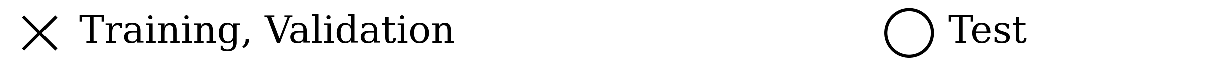
\includegraphics[width=0.6\textwidth]{img/datasets/_legend_theory.pdf}
        \end{subfigure}
        \vspace{-0.2cm} % Add some vertical space between the legend and the subfigures

        \begin{subfigure}[b]{0.17\textwidth}
            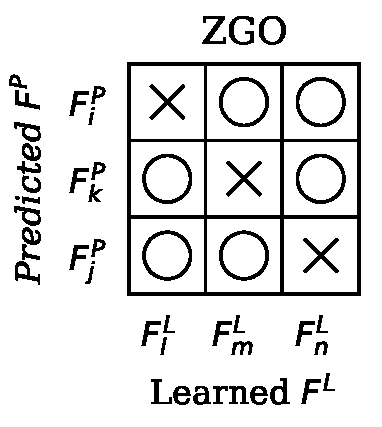
\includegraphics[width=\textwidth]{img/datasets/_ZGO.pdf}
        \end{subfigure}
        \hfill
        \begin{subfigure}[b]{0.17\textwidth}
            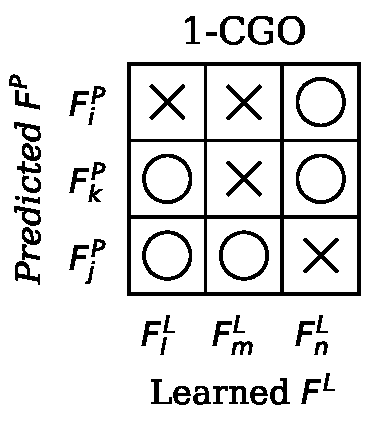
\includegraphics[width=\textwidth]{img/datasets/_1-CGO.pdf}
        \end{subfigure}
        \hfill
        \begin{subfigure}[b]{0.17\textwidth}
            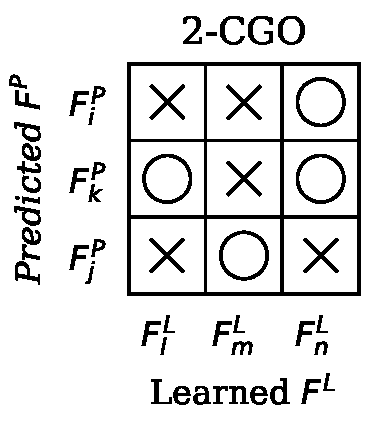
\includegraphics[width=\textwidth]{img/datasets/_2-CGO.pdf}
        \end{subfigure}
        \hfill
        \begin{subfigure}[b]{0.17\textwidth}
            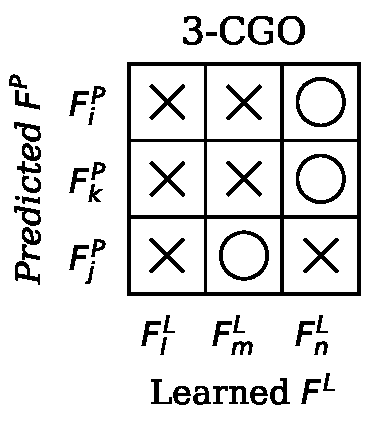
\includegraphics[width=\textwidth]{img/datasets/_3-CGO.pdf}
        \end{subfigure}
        \hfill
        \begin{subfigure}[b]{0.17\textwidth}
            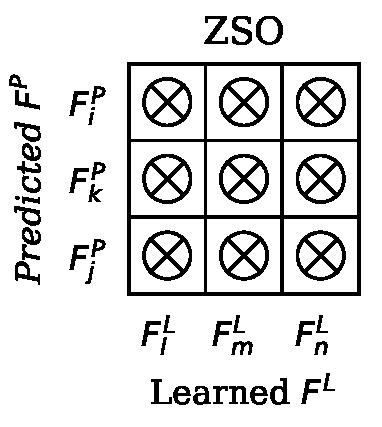
\includegraphics[width=\textwidth]{img/datasets/_ZSO.pdf}
        \end{subfigure}
        
        \caption{Representation of the co-occurrence pattern in between learning factors $F^L$ and predicted
        factors $F^P$ for the ZGO, CGO and ZSO settings that will be considered in this experiment.
        }
    \end{figure}

In this case, only ERM and IRM \cite{arjovskyInvariantRiskMinimization2020}
algorithms will be considered, since data augmentation algorithms such as LISA \cite{yaoImprovingOutofDistributionRobustness2022}
would bypass the synthetically-induced co-occurrence patterns in the datasets, thus preventing a proper 
analysis of the PA model selection capabilities under these specific conditions. These algorithms will be used to 
train a ResNet18 model for 100 epochs using Adam optimizer with learning rates $10^{-2}$ and $10^{-3}$. \\

In order to encompass the primary drivers of inductive bias from a perceptual perspective, these experiments
will be conducted for both hue and position as learning factors $F^L$ and shape as 
the predicted factor $F^P$. The specific configuration of factor values 
and co-occurrence patterns that defines each dataset can be found in Table \ref{def:zgo_experiments}. As has been the case throughout this project, 
test performance will be reported in increasingly shifted test datasets, as specified in Table \ref{tab:sogo_test}. In this case, however,
selected models will be those achieving the highest accuracy in the first test dataset only, which is 
the one assessing the performance in the complementary co-occurring learning factors, and therefore
determining whether the selected model has been able to overcome the limitations posed by the suboptimal
configuration of the data. In total, training, validation and test samples are composed of 30.000, 
15.000 and 3.000 MNIST observations, respectively.\\

Tables \ref{tab:sogo_hue_improve}-\ref{tab:sogo_pos_improve} present the results of this experiment by reporting
the test performance obtained through accuracy-based model selection (Acc) and the improvement in performance obtained
through PA-based model selection ($\Delta$Acc). These results show that PA is able to effectively select models that generalize
better to unseen combinations of factors, particularly in the first environment, for both hue and position factor
experiments. \\

This setting highlights the potential of robustness-driven model selection, as Tables \ref{tab:sogo_hue_full}-\ref{tab:sogo_pos_full}
show that similarly positive results are be obtained with $\operatorname{AFR}_{\text{P}}$ as early stopping criterion. 
Figure \ref{fig:posterior_sogo} and Table \ref{tab:sogo_betas} expand these insights by illustrating
the rationale behind the robustness assessment provided by PA. Under heavy spurious overfitting, mismatch 
between predictions in $\bm{x}_0^{\text{test}}$ and $\bm{x}_1^{\text{test}}$ is very significant, and in most 
cases models are considered to be non-robust. Nevertheless, even when the performance difference between ERM and IRM models 
is minimal, $\beta^{*}$ starts converging to non-zero values at a lower co-occurrence threshold in the
IRM case, if compared to ERM. This underscores the superior robustness-fostering capabilities of IRM.

\begin{table}[H]
    \centering
    \resizebox{\textwidth}{!}{%
    \begin{tabular}{l|cl|cl|cl|cl|cl}
    \multirow{2}{*}{} & \multicolumn{2}{c|}{\textbf{Test 1}} & \multicolumn{2}{c|}{\textbf{Test 2}} & \multicolumn{2}{c|}{\textbf{Test 3}} & \multicolumn{2}{c|}{\textbf{Test 4}} & \multicolumn{2}{c}{\textbf{Test 5}} \\
    \textbf{{\color{tab:blue} \textbf{ERM}}} & Acc. & $\Delta$Acc. & Acc. & $\Delta$Acc. & Acc. & $\Delta$Acc. & Acc. & $\Delta$Acc. & Acc. & $\Delta$Acc. \\
    \midrule
    ZGO & 53.2 & \PlusMinus 0.01 & 54.6 & \PlusMinus 0.01 & 55.7 & \PlusMinus 0.01 & 66.7 & \PlusMinus 0.01 & 66.6 & \PlusMinus 0.01 \\
    1-CGO & 62.9 & {\color{tab:green}  \textbf{\Plus 9.5}} & 64.7 & {\color{tab:green}  \textbf{\Plus 10.2}} & 60.8 & {\color{tab:green}  \textbf{\Plus 0.3}} & 62.9 & {\color{tab:green}  \textbf{\Plus 2.2}} & 64.2 & {\color{tab:green}  \textbf{\Plus 0.5}} \\
    2-CGO & 69.1 & {\color{tab:green}  \textbf{\Plus 9.4}} & 71.2 & {\color{tab:green}  \textbf{\Plus 7.8}} & 71.9 & {\color{tab:green}  \textbf{\Plus 0.3}} & 76.2 & {\color{tab:red} \textbf{\Minus 2.4}} & 77.0 & {\color{tab:red} \textbf{\Minus 2.8}} \\
    3-CGO & 73.1 & {\color{tab:green}  \textbf{\Plus 16.6}} & 85.6 & {\color{tab:green}  \textbf{\Plus 3.6}} & 70.1 & {\color{tab:green}  \textbf{\Plus 9.7}} & 71.4 & {\color{tab:green}  \textbf{\Plus 6.4}} & 72.1 & {\color{tab:green}  \textbf{\Plus 6.7}} \\
    ZSO & 99.6 & \PlusMinus 0.01 & 92.8 & {\color{tab:red} \textbf{\Minus 0.1}} & 89.9 & {\color{tab:green}  \textbf{\Plus 0.2}} & 85.9 & \PlusMinus 0.01 & 85.9 & \PlusMinus 0.01 \\
    \midrule
    \addlinespace
    \addlinespace
    \textbf{{\color{tab:orange} \textbf{IRM}}} & Acc. & $\Delta$Acc. & Acc. & $\Delta$Acc. & Acc. & $\Delta$Acc. & Acc. & $\Delta$Acc. & Acc. & $\Delta$Acc. \\
    \midrule
    ZGO & 50.1 & {\color{tab:green}  \textbf{\Plus 5.9}} & 50.5 & {\color{tab:green}  \textbf{\Plus 4.9}} & 52.8 & {\color{tab:green}  \textbf{\Plus 9.5}} & 64.4 & {\color{tab:green}  \textbf{\Plus 1.1}} & 64.9 & {\color{tab:green}  \textbf{\Plus 1.2}} \\
    1-CGO & 63.0 & {\color{tab:green}  \textbf{\Plus 7.0}} & 65.9 & {\color{tab:green}  \textbf{\Plus 7.6}} & 59.4 & {\color{tab:green}  \textbf{\Plus 2.2}} & 60.1 & {\color{tab:green}  \textbf{\Plus 2.2}} & 59.0 & {\color{tab:green}  \textbf{\Plus 1.8}} \\
    2-CGO & 69.0 & {\color{tab:green}  \textbf{\Plus 10.6}} & 69.7 & {\color{tab:green}  \textbf{\Plus 10.0}} & 67.5 & {\color{tab:green}  \textbf{\Plus 4.7}} & 64.5 & {\color{tab:green}  \textbf{\Plus 13.0}} & 65.1 & {\color{tab:green}  \textbf{\Plus 12.6}} \\
    3-CGO & 79.5 & {\color{tab:green}  \textbf{\Plus 11.6}} & 83.0 & {\color{tab:green}  \textbf{\Plus 9.8}} & 73.6 & {\color{tab:green}  \textbf{\Plus 10.9}} & 70.7 & {\color{tab:green}  \textbf{\Plus 11.0}} & 72.2 & {\color{tab:green}  \textbf{\Plus 11.3}} \\
    ZSO & 99.4 & {\color{tab:green}  \textbf{\Plus 0.1}} & 93.4 & {\color{tab:green}  \textbf{\Plus 1.3}} & 89.2 & {\color{tab:green}  \textbf{\Plus 0.2}} & 87.0 & {\color{tab:green}  \textbf{\Plus 1.6}} & 87.0 & {\color{tab:green}  \textbf{\Plus 1.6}} \\
    \bottomrule
    \end{tabular}%
    }
    \caption{
        Test performance under increasing levels of shift for models selected through different configurations of factor
        co-occurrence for the hue learning factor experiment. Specifically, the performance of models selected through validation accuracy (Acc) and
        the difference between accuracy-based and PA-based selection ($\Delta$Acc) is reported. PA is able to select models
        that perform better than the one selected through accuracy in the most cases. 
    }
    \label{tab:sogo_hue_improve}
\end{table}

\begin{table}[H]
    \centering
    \resizebox{\textwidth}{!}{%
    \begin{tabular}{l|cl|cl|cl|cl|cl}
    \multirow{2}{*}{} & \multicolumn{2}{c|}{\textbf{Test 1}} & \multicolumn{2}{c|}{\textbf{Test 2}} & \multicolumn{2}{c|}{\textbf{Test 3}} & \multicolumn{2}{c|}{\textbf{Test 4}} & \multicolumn{2}{c}{\textbf{Test 5}} \\
    \textbf{{\color{tab:blue} \textbf{ERM}}} & Acc. & $\Delta$Acc. & Acc. & $\Delta$Acc. & Acc. & $\Delta$Acc. & Acc. & $\Delta$Acc. & Acc. & $\Delta$Acc. \\
    \midrule
    ZGO & 50.2 & \PlusMinus 0.01 & 50.0 & \PlusMinus 0.01 & 52.4 & \PlusMinus 0.01 & 52.0 & \PlusMinus 0.01 & 50.6 & \PlusMinus 0.01 \\
    1-CGO & 44.1 & {\color{tab:green}  \textbf{\Plus 4.2}} & 41.4 & {\color{tab:green}  \textbf{\Plus 0.5}} & 43.6 & {\color{tab:green}  \textbf{\Plus 1.5}} & 45.0 & {\color{tab:green}  \textbf{\Plus 1.0}} & 44.8 & {\color{tab:green}  \textbf{\Plus 1.2}} \\
    2-CGO & 64.4 & {\color{tab:green}  \textbf{\Plus 7.0}} & 53.4 & {\color{tab:green}  \textbf{\Plus 1.7}} & 55.1 & {\color{tab:green}  \textbf{\Plus 2.7}} & 57.7 & {\color{tab:green}  \textbf{\Plus 1.3}} & 56.7 & {\color{tab:green}  \textbf{\Plus 1.3}} \\
    3-CGO & 73.2 & {\color{tab:green}  \textbf{\Plus 17.9}} & 55.3 & {\color{tab:green}  \textbf{\Plus 8.3}} & 52.8 & {\color{tab:green}  \textbf{\Plus 8.5}} & 51.8 & {\color{tab:green}  \textbf{\Plus 7.0}} & 51.8 & {\color{tab:green}  \textbf{\Plus 7.2}} \\
    ZSO & 99.1 & \PlusMinus 0.01 & 92.1 & {\color{tab:red} \textbf{\Minus 0.2}} & 88.6 & {\color{tab:green}  \textbf{\Plus 0.2}} & 87.0 & {\color{tab:green}  \textbf{\Plus 0.1}} & 85.7 & {\color{tab:green}  \textbf{\Plus 0.2}} \\
    \midrule
    \addlinespace
    \addlinespace
    \textbf{{\color{tab:orange} \textbf{IRM}}} & Acc. & $\Delta$Acc. & Acc. & $\Delta$Acc. & Acc. & $\Delta$Acc. & Acc. & $\Delta$Acc. & Acc. & $\Delta$Acc. \\
    \midrule
    ZGO & 50.5 & \PlusMinus 0.01 & 50.0 & \PlusMinus 0.01 & 53.1 & \PlusMinus 0.01 & 52.5 & \PlusMinus 0.01 & 51.6 & \PlusMinus 0.01 \\
    1-CGO & 48.2 & {\color{tab:green}  \textbf{\Plus 0.8}} & 43.6 & {\color{tab:green}  \textbf{\Plus 0.6}} & 43.2 & {\color{tab:red} \textbf{\Minus 0.4}} & 44.0 & {\color{tab:red} \textbf{\Minus 1.7}} & 44.1 & {\color{tab:red} \textbf{\Minus 2.1}} \\
    2-CGO & 65.0 & {\color{tab:green}  \textbf{\Plus 7.1}} & 53.1 & {\color{tab:green}  \textbf{\Plus 5.6}} & 52.8 & {\color{tab:green}  \textbf{\Plus 1.3}} & 59.2 & {\color{tab:red} \textbf{\Minus 3.7}} & 60.1 & {\color{tab:red} \textbf{\Minus 4.7}} \\
    3-CGO & 80.4 & {\color{tab:green}  \textbf{\Plus 13.8}} & 63.2 & {\color{tab:green}  \textbf{\Plus 7.7}} & 57.5 & {\color{tab:green}  \textbf{\Plus 6.0}} & 51.4 & {\color{tab:green}  \textbf{\Plus 7.4}} & 52.6 & {\color{tab:green}  \textbf{\Plus 5.2}} \\
    ZSO & 99.6 & {\color{tab:red} \textbf{\Minus 0.3}} & 93.8 & {\color{tab:red} \textbf{\Minus 1.0}} & 88.2 & {\color{tab:red} \textbf{\Minus 2.5}} & 89.5 & {\color{tab:red} \textbf{\Minus 8.1}} & 89.6 & {\color{tab:red} \textbf{\Minus 8.4}} \\
    \bottomrule
    \end{tabular}%
    }
    \caption{
        Test performance under increasing levels of shift for models selected through different configurations of factor
        co-occurrence for the position learning factor experiment. Specifically, the performance of models selected through validation accuracy (Acc) and
        the difference between accuracy-based and PA-based selection ($\Delta$Acc) is reported. PA is able to select models
        that perform better than the one selected through accuracy in the most cases.
    }
    \label{tab:sogo_pos_improve}
    \end{table}

\begin{figure}[H]
    \centering
    \begin{subfigure}[b]{0.45\textwidth}
        \centering
        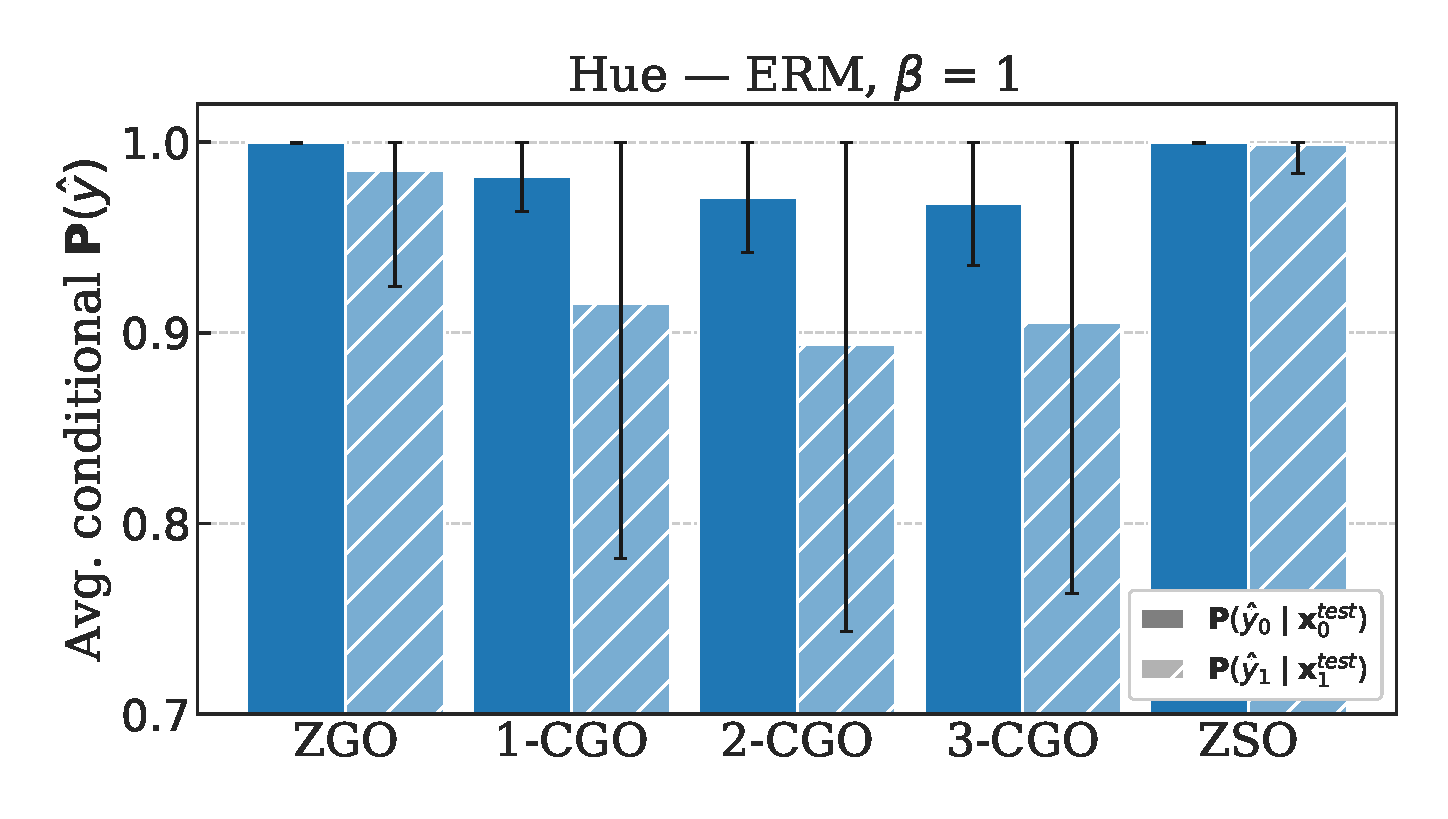
\includegraphics[width=\textwidth]{img/model_selection/posterior_erm_hue.pdf}
    \end{subfigure}
    \hfill
    \begin{subfigure}[b]{0.45\textwidth}
        \centering
        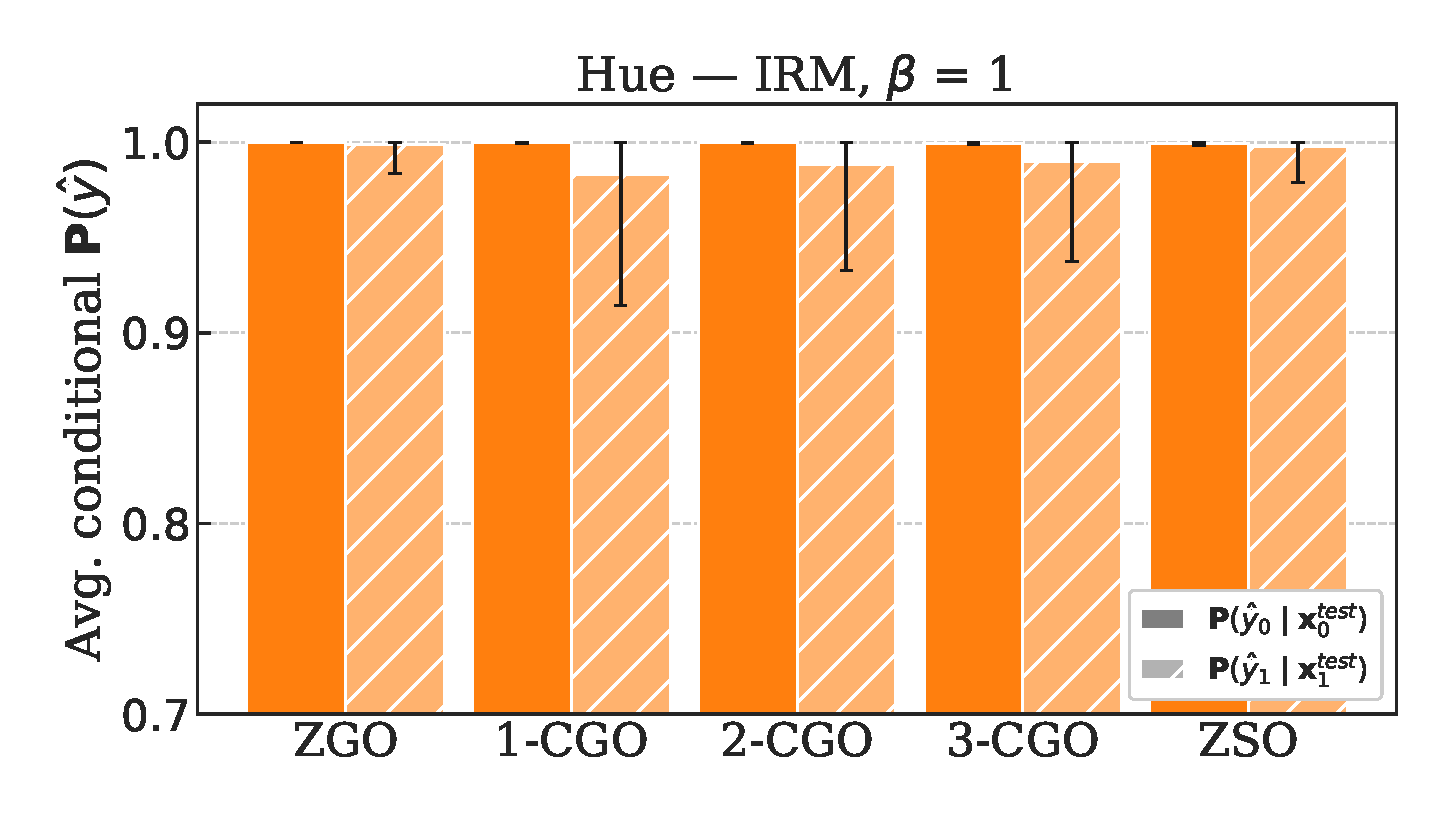
\includegraphics[width=\textwidth]{img/model_selection/posterior_irm_hue.pdf}
    \end{subfigure}

    \vspace{1em}

    \begin{subfigure}[b]{0.45\textwidth}
        \centering
        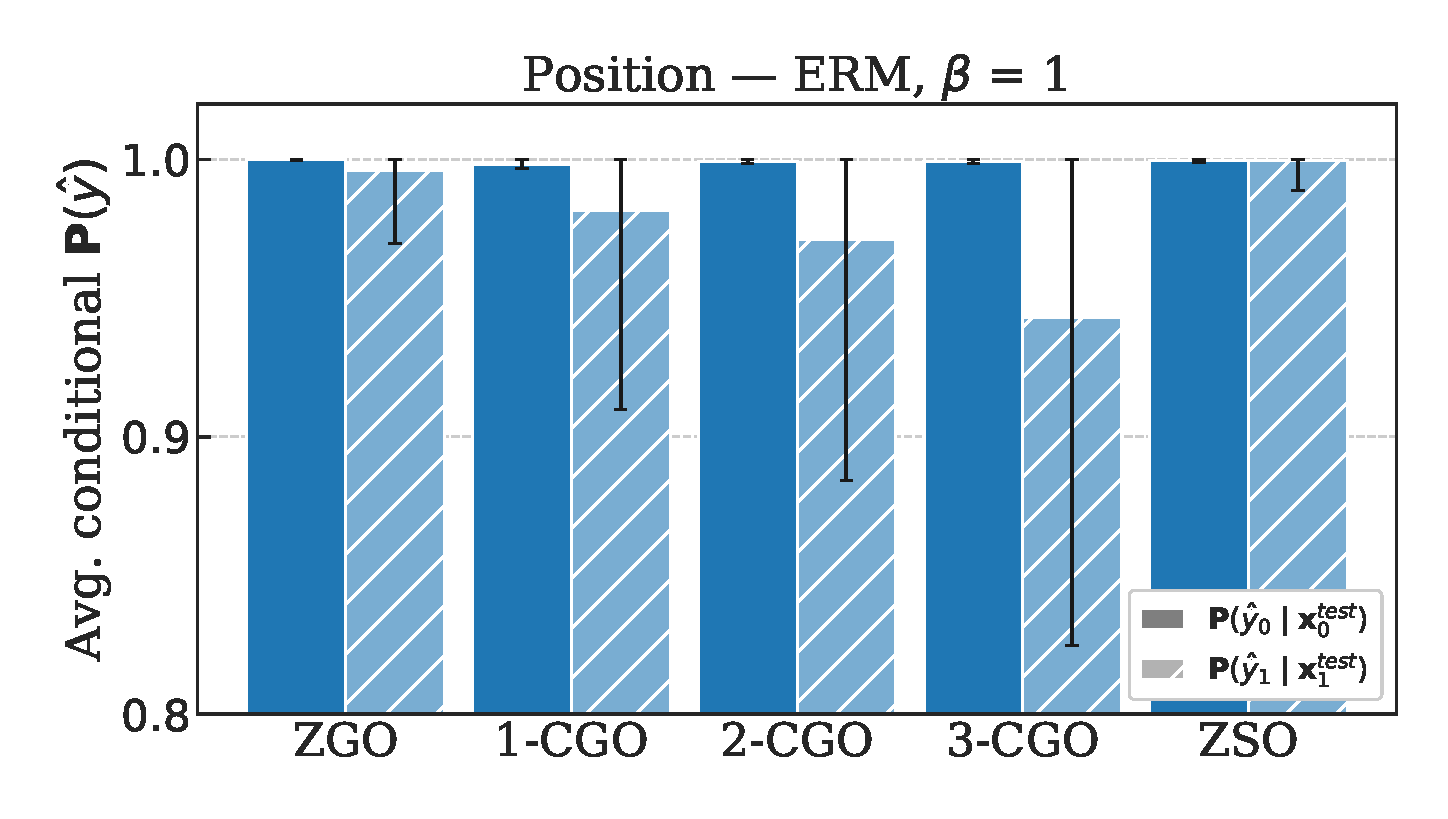
\includegraphics[width=\textwidth]{img/model_selection/posterior_erm_position.pdf}
    \end{subfigure}
    \hfill
    \begin{subfigure}[b]{0.45\textwidth}
        \centering
        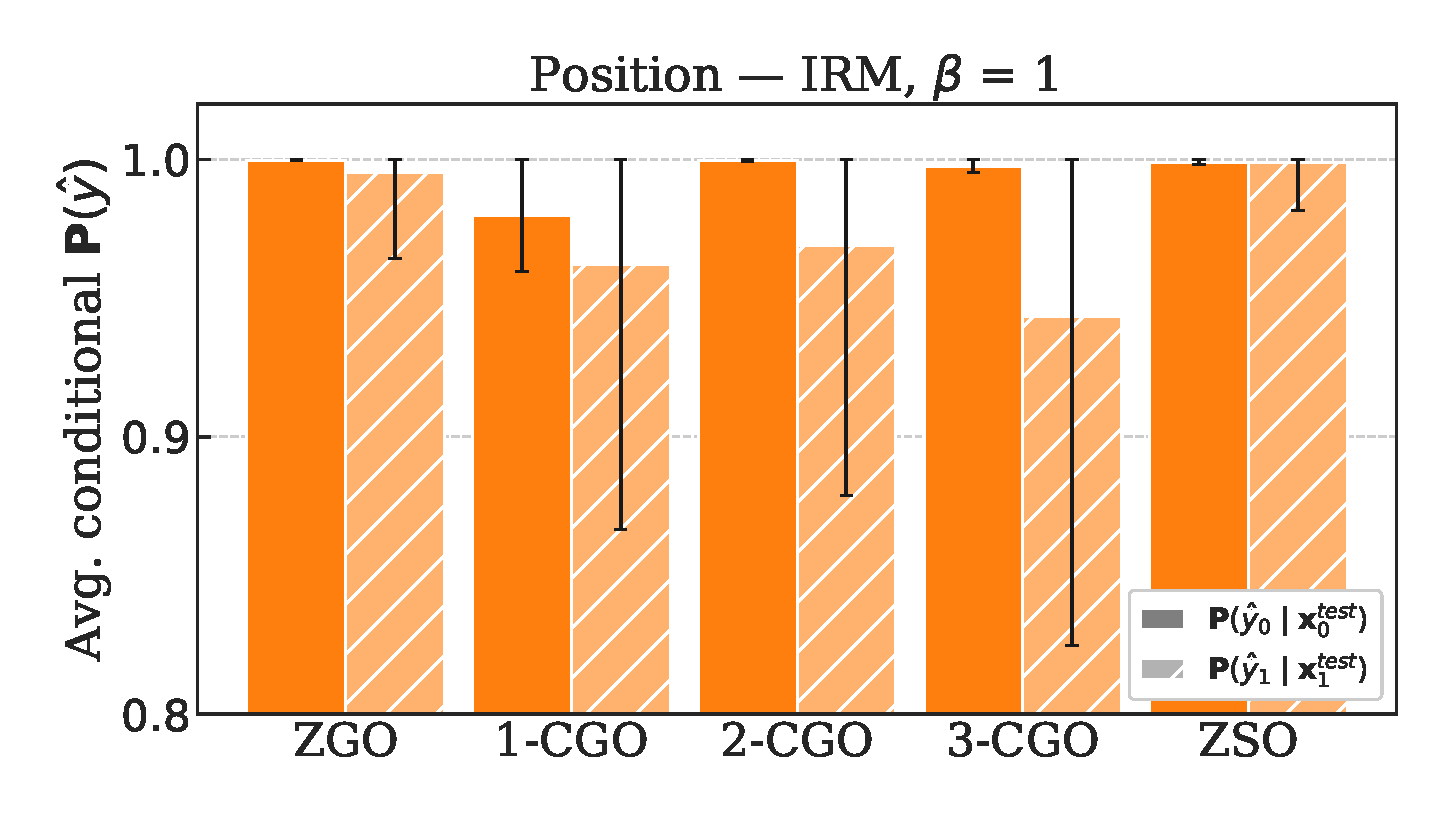
\includegraphics[width=\textwidth]{img/model_selection/posterior_irm_position.pdf}
    \end{subfigure}

    \caption{
    Average posterior distribution at the predicted class for the different ZGO, CGO and ZSO settings
    for the hue and position learning factor experiments. The posterior distribution is computed
    for the first test dataset, which is the one assessing the performance in the complementary co-occurring
    learning factors. 
    }
    \label{fig:posterior_sogo}
\end{figure}

\begin{table}[H]
    \centering
    \begin{tabular}{l|c|c|c|c|c}
    Hue & \textbf{ZGO} & \textbf{1-CGO} & \textbf{2-CGO} & \textbf{3-CGO} & \textbf{ZSO}\\
    \midrule
    \textbf{{\color{tab:blue} \textbf{ERM}}}   & 0.000  & 0.000  & 0.000  & 0.000  & 85.98  \\
    \textbf{{\color{tab:orange} \textbf{IRM}}}  & 0.000  & 0.000  & 2.110 & 17.34 & 116.3   \\
    \midrule
    \addlinespace
    \addlinespace
    position & \textbf{ZGO} & \textbf{1-CGO} & \textbf{2-CGO} & \textbf{3-CGO} & \textbf{ZSO}\\
    \midrule
    \textbf{{\color{tab:blue} \textbf{ERM}}}   & 0.000 & 0.000  & 0.000  & 0.000  & 1720    \\
    \textbf{{\color{tab:orange} \textbf{IRM}}}  & 0.000 & 0.000  & 3.984  & 34.107  & 2254     \\
    \bottomrule
    \end{tabular}
    \caption{
        A comparison of the $\beta^{*}$ values obtained in \textbf{Experiment 7} reveals that ERM 
        models are entirely non-robust up until the ZSO setting, whereas IRM models demonstrate 
        generalization capabilities (i.e. $\beta^{*}> 1$) starting from the 1-CGO setting. 
    }
    \label{tab:sogo_betas}
\end{table}


 \section{WILDS Benchmark}

In light of the results obtained in this chapter, the model selection 
capabilities of PA will be finally assessed on standard benchmark datasets in out-of-distribution settings. 
In particular, several WILDS \cite{kohWILDSBenchmarkIntheWild2021} 
datasets will be considered, as they offer a comprehensive set of domain generalization 
tasks that is representative of real-world scenarios and are widely used in the literature to report 
performance in robust learning. \\

Every dataset under consideration entails a specific configuration of 
learning opportunities that will shift the inductive bias towards suboptimal representations. The domain 
generalization performance of the models will be assessed on target domains and the selection capabilities of
the different metrics will be compared. In particular, only domain adaptation settings 
will be considered, as PA has been proven to consistently outperform accuracy-based metrics 
in these conditions. \\

Every experiment is associated to a specific WILDS dataset, where the data configuration, network architecture
and  optimization settings were drawn from either the original publication or from the configurations specified for 
IRM \cite{arjovskyInvariantRiskMinimization2020} and 
LISA \cite{yaoImprovingOutofDistributionRobustness2022} algorithms in their respective works. 
To ensure consistency, the setup and construction of the required environments strictly adhered to the 
guidelines outlined in these publications. \\

With regard to PA model selection, it must be noted that samples associated to each domain in
the validation set were initially not sorted or paired in any way. For the purpose of these experiments, and given
the results obtained in previous sections, observations from validation samples $\bm{x}_0^{\text{val}}, \bm{x}_1^{\text{val}}$
were paired by performing a nearest-neighbour search in the feature space after the first training epoch, conditioned on class membership. In that way,
posterior agreement would be computed in a similar setting to the one considered in the synthetic experiments, under both 
sampling randomness (even if not entirely random due to the pairing) and domain shift. This pairing method is clearly
suboptimal, as it is biased by the specific representation of features delivered after the first training epoch. However, it was selected for
efficiency purposes, and it was conducted using the L2 Euclidean distance implementation of the FAISS \cite{faiss} library.

\paragraph{Experiment 8.} The \textbf{waterbirds} dataset was considered. The classification task involves the prediction of
two classes of birds, namely \texttt{waterbird} and \texttt{landbird}. The dataset is balanced in the classes of birds, but images encode a
spurious correlation that arises from their different habitats. In particular, the configuration considered in this experiment is such that
the background of the images is unbalanced in the train dataset, which contains 3554 images with water background and only 1241 images
with land background. Both validation and test datasets are balanced, and the shortcut opportunity encoded by the background subpopulation
shift will be exploited. More specifically, source domains will be defined from the background type, and robustness and performance in between
these will be considered as model selection criteria.

\paragraph{Experiment 9.} The \textbf{celebA} dataset was considered. The classification task involves the prediction
of hair color from images of American celebrities, namely \texttt{blonde} and \texttt{not blonde}. The subpopulation shift arises from
the spurious correlation existing between the gender of the celebrity and the color of their hair. In particular, 
Table \ref{tab:celebA_freqtable} contains the relative frequency of the gender-hair color combinations in the training dataset. 
Source domains will be defined from the hair color (i.e. the label), and robustness and performance in between
these will be considered as model selection criteria.

\begin{table}[H]
    \centering
    \begin{tabular}{l|c|c}
    & \texttt{blonde} & \texttt{not blonde} \\
    \midrule
    Male   & 1741   & 89931  \\
    Female & 28234   & 82685   \\
    \bottomrule
    \end{tabular}
    \caption{
        Relative frequency of the gender-hair color combinations in the \texttt{celebA} \cite{kohWILDSBenchmarkIntheWild2021} dataset.
        The \texttt{blonde} class is underrepresented, especially in male pictures.
    }
    \label{tab:celebA_freqtable}
\end{table}

\paragraph{Experiment 10.} The \textbf{camelyon17} dataset was considered. The classification task involves the identification of tumor
tissue in lymph node patches sampled from different hospitals, which amounts to the classes \texttt{tumor} and \texttt{no tumor}. 
The out-of-distribution setting originates from the differences in the samples taken from different hospitals, as illustrated in Figure \ref{fig:camelyon17}. 
In particular, the composition of the training, validation and test datasets is specified in Table \ref{tab:camelyon17_idval}.
Each of the three first hospitals defines a source environment, and the generalization capabilities over observations in the fourth hospital will be examined.

\begin{table}[H]
    \centering
    \begin{tabular}{l|c|c|c|c}
    Hospital & 1 & 2 & 3 & 4 \\
    \midrule
    Training   & 53425 & 116959 & 132052 & - \\
    Validation & 6011  & 12879  & 14670 & -\\
    Test & - & - & - & 85054 \\
    \bottomrule
    \end{tabular}
    \caption{
        Hospital of origin of the lymph node patches that compose training, validation and test datasets in the \texttt{camelyon17} \cite{kohWILDSBenchmarkIntheWild2021} dataset.
    }
    \label{tab:camelyon17_idval}
\end{table}

\begin{table}[H]
    \centering
    \setlength{\tabcolsep}{2.5pt}
    \begin{tabular}{l|ccc|ccc}
    \multirow{3}{*}{} & \multicolumn{3}{c|}{\textbf{Average Acc.}} & \multicolumn{3}{c}{\textbf{Worst-case Acc.}}\\
    & Acc. & AFR$_\text{P}$ & PA & Acc. & AFR$_\text{P}$ & PA \\
    \midrule
    \textbf{{\color{tab:blue} \textbf{ERM}}} & \textbf{78.52} & 73.72 & \textbf{78.52} & \textbf{67.11} & 58.90 & \textbf{67.11} \\
    \textbf{{\color{tab:orange} \textbf{IRM}}} & \textbf{90.16} & 89.70 & \textbf{90.16} & \textbf{89.21} & 88.67 & \textbf{89.21} \\
    \bottomrule
    \end{tabular}
    \caption{
        Average and worst-case test accuracy for the \texttt{waterbirds} \cite{kohWILDSBenchmarkIntheWild2021} dataset.
        PA outperforms AFR$_\text{P}$ due to the vulnerability of the latter to the specific sampling instantiation. More specifically,
        while PA has a monotonically increasing evolution during training, AFR$_\text{P}$ is only monotonic in mean, and the variation
        around the mean at every epoch hinders its selection consistency.
    }
    \label{tab:waterbirds}
\end{table}

\begin{table}[H]
    \centering
    \setlength{\tabcolsep}{2.5pt}
    \begin{tabular}{l|ccc|ccc}
    \multirow{3}{*}{} & \multicolumn{3}{c|}{\textbf{Average Acc.}} & \multicolumn{3}{c}{\textbf{Worst-case Acc.}}\\
     & Acc. & AFR$_\text{P}$ & PA & Acc. & AFR$_\text{P}$ & PA \\
    \midrule
    \textbf{{\color{tab:blue} \textbf{ERM}}} & 97.80 & \textbf{98.27} & \textbf{98.27} & 97.76 & \textbf{97.77} & \textbf{97.77}\\
    \textbf{{\color{tab:orange} \textbf{IRM}}} & 98.12 & \textbf{98.41} & \textbf{98.41} & \textbf{98.06} & 98.05 & 98.05 \\
    \bottomrule
    \end{tabular}
    \caption{
        Average and worst-case test accuracy for the \texttt{celebA} \cite{kohWILDSBenchmarkIntheWild2021} dataset. Robustness-based
        selection metrics outperform accuracy in most cases.
    }
    \label{tab:celebA}
\end{table}

\begin{table}[H]
    \centering
    \setlength{\tabcolsep}{2.5pt}
    \begin{tabular}{l|ccc}
    \multirow{3}{*}{} & \multicolumn{3}{c}{\textbf{Accuracy}} \\
     & Acc. & AFR$_\text{P}$ & PA \\
    \midrule
    \textbf{{\color{tab:blue} \textbf{ERM}}} & 86.73 & 86.73 & 86.73 \\
    \textbf{{\color{tab:orange} \textbf{IRM}}} & 67.98 & 67.98 & 67.98 \\
    \textbf{{\color{tab:green} \textbf{LISA}}} & 81.1 & \textbf{81.8} & \textbf{81.8} \\
    \bottomrule
    \end{tabular}
    \caption{
        Test accuracy for the \texttt{camelyon17} \cite{kohWILDSBenchmarkIntheWild2021} dataset.
        No significant improvement is observed, with the exception of the LISA model.
    }
    \label{tab:camelyon17}
    \end{table}

Tables \ref{tab:waterbirds}-\ref{tab:camelyon17} display the average performance and worst-case performance (when 
applicable) obtained on test datasets for the different model selection criteria. Overall, PA-based model selection 
shows the best results, as it is consistently able to select models that generalize better to test data, while 
accuracy and AFR$_\text{P}$ are shown to underperform in some settings. However promising, 
these results should be taken with caution and further experimentation should be pursued to fully determine the 
generalizability of this approach to other datasets and other possible configurations of source domains. \\

 \cleardoublepage